% Author: Izaak Neutelings (March, 2017)
\documentclass[border=3pt,tikz]{standalone} %[dvipsnames]
\usepackage{amsmath} % for \dfrac
\usepackage{siunitx,physics}
\usepackage{tikz}
\tikzset{>=latex} % for LaTeX arrow head
\usepackage{pgfplots} % for the axis environment
%\usepackage[outline]{contour} % halo around text
%\contourlength{1.2pt}
\usepackage{xcolor}
\colorlet{mygreen}{green!60!black}
\colorlet{myblue}{blue!70!black}
\colorlet{myred}{red!70!black}
\tikzstyle{rline}=[myred,thick]
\tikzstyle{bline}=[myblue,thick]
\tikzstyle{gline}=[mygreen,thick]
\pgfplotsset{compat=1.13} % TikZ coordinates <-> axes coordinates
%\pgfplotsset{compat=1.17}
\colorlet{mydarkblue}{blue!30!black}
\def\N{50}

% H2:  4u/2k =  4*1.66*10^(-27)/(2*1.38*10^(-23)) = 0.00024
% O2: 32u/2k = 32*1.66*10^(-27)/(2*1.38*10^(-23)) = 0.00192
% 4/sqrt(pi)
%\def\k{0.00024}
\pgfmathdeclarefunction{maxwell}{2}{%
  \pgfmathparse{4/sqrt(pi)*(\k/#2)^(3/2)*(#1^2)*exp(-\k*(#1^2)/#2)}%
}
\def\maxwell#1#2{4/sqrt(pi)*(\k/#2)^(3/2)*((\xscale*#1)^2)*exp(-((\xscale*#1)^2)*(\k/#2))}
%\def\vmax#1{sqrt(#1/\k)/\xscale}
\def\tick#1#2{\draw[thick] (#1) ++ (#2:0.03*\ymax) --++ (#2-180:0.06*\ymax)}


\begin{document}



% MAXWELL-BOLTZMANN different temperatures
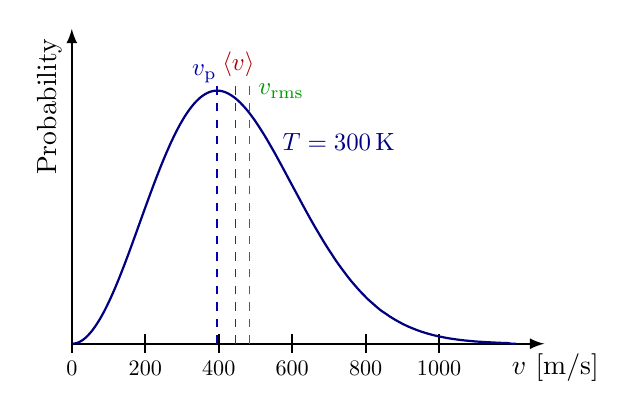
\begin{tikzpicture}
  \def\xmax{6.0}
  \def\ymax{4.0}
  \def\k{4500} % k = m/2k
  \def\xscale{0.14}
  \def\vn{2.6}
  \def\vmax{sqrt(300/\k)/\xscale}
  \def\vrms{sqrt(300/(2*\k/3))/\xscale}
  \def\vave{2*\vmax/sqrt(pi)}
  \coordinate (O) at (0,0);
  \coordinate (X) at (\xmax,0);
  \coordinate (Y) at (0,\ymax);
  
  % AXIS
  \draw[<->,thick]
    (Y) node[above left,rotate=90] {Probability} -- (0,0) -- (X) node[right=4,below] {$v$ [\si{m/s}]};
  \foreach %\x [evaluate={\c=sqrt(\k/0.00096); \v=(round(\x*\c/\xscale))}] in {1,...,3}{
           \i [evaluate={\v=int(\i*200);}] in {0,...,5}{
    \pgfmathsetmacro\x{\v*sqrt(0.00192)/\xscale/sqrt(\k))} % higher precision
    \tick{\x,0}{90} node[below,scale=0.8] {\v};
  }
  
  % LABELS
  \node[blue!50!black,above right=-1,scale=0.9] at (\vn,{\maxwell{\vn}{300}}) {$T=\SI{300}{K}$}; %f(x)
  \draw[myblue,dashed,thin]
    ({\vmax},0) coordinate (VM) --++ (0,{1.04*\maxwell{\vmax}{300}})
    node[myblue,left=1,above left=-4,scale=0.9] {$v_\text{p}$};
  \draw[myred,dashed,thin]
    ({\vave},0) coordinate (VA) --++ (0,{1.04*\maxwell{\vmax}{300}})
    node[myred,right=1,above=-2,scale=0.9] {$\expval{v}$};
  \draw[mygreen,dashed,thin]
    ({\vrms},0) coordinate (VR) --++ (0,{1.04*\maxwell{\vmax}{300}})
    node[mygreen,above=2,below right=0,scale=0.9] {$v_\text{rms}$};
  %\tick{VM}{90}; %node[myblue,right=1,below left=0,scale=0.85] {$v_\text{p}$};
  %\tick{VA}{90}; %node[myred,left=1,below=-2,scale=0.85] {$\expval{v}$};
  %\tick{VR}{90}; %node[mygreen,below right=0,scale=0.85] {$v_\text{rms}$};
  
  % PLOT
  \draw[blue!50!black,thick,samples=100,smooth,variable=\x,domain=0.01:0.94*\xmax]
    plot(\x,{\maxwell{\x}{300}});
  
\end{tikzpicture}



% MAXWELL-BOLTZMANN different temperatures
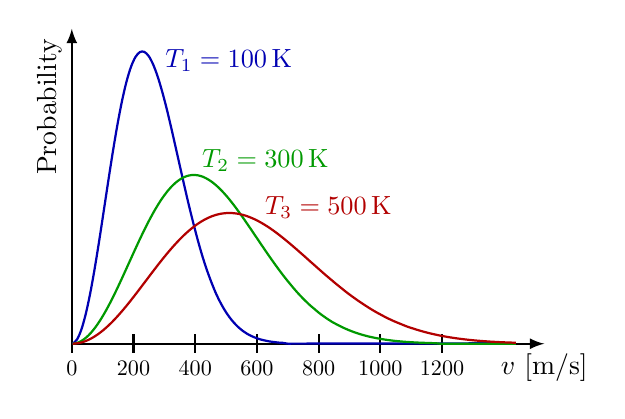
\begin{tikzpicture}
  \def\xmax{6.0}
  \def\ymax{4.0}
  \def\k{2000}
  \def\xscale{0.25}
  \def\vb{1.1}
  \def\vg{1.6}
  \def\vr{2.4}
  \coordinate (O) at (0,0);
  \coordinate (X) at (\xmax,0);
  \coordinate (Y) at (0,\ymax);
  
  % AXIS
  \draw[<->,thick]
    (Y) node[above left,rotate=90] {Probability} -- (0,0) -- (X) node[below] {$v$ [\si{m/s}]};
  \foreach \i [evaluate={\v=int(\i*200);}] in {0,...,6}{
    \pgfmathsetmacro\x{\v*sqrt(0.00192)/\xscale/sqrt(\k))} % higher precision
    \tick{\x,0}{90} node[below,scale=0.8] {\v};
  }
  
  % LABELS
  \node[bline,above right=-1,scale=0.95] at (\vb,{\maxwell{\vb}{100}}) {$T_1=\SI{100}{K}$};
  \node[gline,above right=-2,scale=0.95] at (\vg,{\maxwell{\vg}{300}}) {$T_2=\SI{300}{K}$};
  \node[rline,above right=-2,scale=0.95] at (\vr,{\maxwell{\vr}{500}}) {$T_3=\SI{500}{K}$};
  
  % PLOT
  \draw[bline,samples=100,smooth,variable=\x,domain=0.01:0.94*\xmax]
    plot(\x,{\maxwell{\x}{100}});
  \draw[gline,samples=100,smooth,variable=\x,domain=0.01:0.94*\xmax]
    plot(\x,{\maxwell{\x}{300}});
  \draw[rline,samples=100,smooth,variable=\x,domain=0.01:0.94*\xmax]
    plot(\x,{\maxwell{\x}{500}});
  
\end{tikzpicture}






%% MAXWELL-BOLTZMANN with axes
%\begin{tikzpicture}
%  
%  \def\N{40};
%  \def\k{0.00024}
%  \def\vmax{sqrt(300/\k)};
%  \def\xmin{0};
%  \def\xmax{4e3};
%  \def\ymax{1.15*maxwell(\vmax,300)};
%  
%  \begin{axis}[every axis plot post/.append style={
%               mark=none,domain=0:\xmax,samples=\N,smooth},
%               xmin={-0.1*\xmax}, xmax={1.05*\xmax},
%               ymin={-0.1*\ymax}, ymax={\ymax},
%               restrict y to domain=0:\ymax,
%               axis lines=middle,
%               axis line style=thick,
%               %enlargelimits=upper, % extend the axes a bit to the right and top
%               tick style={black,thick},
%               ticklabel style={scale=0.8},
%               xtick style={draw=none}, xticklabels=none,
%               %ticks=none,
%               tick scale binop=\times,
%               %every y tick scale label/.style={at={(rel axis cs:0,1)},anchor=south}
%               xlabel={$v$ [m/s]},
%               ylabel={probability},
%               xlabel style={at={(rel axis cs:-0.1,0.5)},above=50pt,font=\small},
%               ylabel style={at={(rel axis cs:-0.1,0.5)},rotate=90},
%               every axis x label/.style={at={(current axis.right of origin)},anchor=north},
%               width=0.7*\textwidth, height=0.55*\textwidth,
%               %clip=false
%              ]
%    
%    % PLOTS
%    \addplot[blue,thick] {maxwell(x,300)};
%    \addplot[blue,thick] {maxwell(x,400)};
%    
%    % LINES
%    \addplot[mydarkblue,dashed,thick]
%      coordinates {({\vmax},{.95*\ymax}) ({\vmax},{0})} %-.05*(\ymax)
%      node[mydarkblue,below=-2pt] {$v_\text{max}$};
%    
%  \end{axis}
%\end{tikzpicture}


\end{document}
